\documentclass[11pt]{article}

\usepackage[margin = 0.5 in]{geometry}
\usepackage[pdftex]{graphicx}
\graphicspath{{images/}}
\usepackage{subfigure}
\usepackage{booktabs}
\usepackage{multirow}
\usepackage[table]{xcolor}
\usepackage{array}
%\usepackage{amsmath}
\usepackage{booktabs}
\usepackage{multirow}
\usepackage{amsmath}
\usepackage{url}
\usepackage[colorlinks=true,urlcolor=blue]{hyperref}
\renewcommand\UrlFont{\color{blue}}


\title{Datathon Group 3}
\author{ Johnathan Salamanca, Mario Cer\'{o}n, \\
Carol Martinez, Javier Cocunubo, Jairo Nino, Alvaro Munoz
 }
\date{\today}

\begin{document}
\maketitle

\begin{abstract}

In this document the project scope and plan for the Datathon are presented. The document provides information of the data cleaning process and some plots with preliminar results of the data wrangling process.


\end{abstract}

%\section{Introduction}
%You are asked to explore the
%provided data and based on this, pose a question which you believe would be interesting to
%answer. You and your team will then write a report detailing why you believe this question is
%important and how you went about answering it.


\section{Project Scoping \& Plan}
\label{sec:app}

\subsection{Scope}


\begin{itemize}

\item \textbf{Project Objective:}
\begin{itemize}
\item \textbf{Main question}: \textit{How do yellow cabs mean trip distance have changed over time (rush/non-rush hours) as a result of Uber's trips growth?} \\ 
\textit{What are the patterns related to unattended areas of public service?} \\ 

%sFrom this one we can analyze the mean income of the zones where yellow cabs drop-off zones changed.
\end{itemize}

\item \textbf{Main stakeholders}: the NYC citizen and government, and transportation industry (at all levels).

\item \textbf{Boundaries of the project}:

\begin{itemize}
%\item We do not offer forecasts or modeling/ infer data.
\item We will show metrics of the impact of Uber incursion in NYC over the other transportation means.
\item The analysis will be made only on the information of the NYC Boroughs.
%\item We do not offer recommendations, only do support to decision making process for the stakeholders.
\end{itemize}

\item \textbf{Risks:} 
\begin{itemize}
\item Data quality issues in the datasets.
\item The data might be not sufficient to answer the proposed question. 
\end{itemize}

\end{itemize}


\subsection{Plan}
\begin{itemize}
\item \textbf{Summary}: \textit{How do yellow cabs mean trip distance have changed over time (rush/non-rush hours) as a result of Uber's trips growth?}  From this one we can analyze the mean income of the zones where yellow cabs drop-off zones changed.


\item \textbf{Expected Deliverable}: A report with the topic question, Data wrangling and Cleaning process, Exploratory Data Analysis EDA, Statistical Analysis and Modeling, Results Interpretation and Conclusions.

\item \textbf{How to get there}: 
\begin{itemize}
\item Clean, wrangled and analyze the dataset.
\item Conduct exploratory data analysis.
\item Conduct Analysis \& modeling.
\item Conclusions and final report (source code and power point presentation).
\end{itemize}

\end{itemize}

%\section{Topic Question}
%\abel{sec:topicQ}
%What is the question that your team set out to answer? How did you
%come about to choosing this question, and why is it an important question?
\section{Introduction}
\label{sec:Intro}
Introduction section of final report written.
This should clearly state the context of your team?s application and the problem you set out to solve, as well as your justification for why it is an important problem.

\section{Data Wrangling and Data Cleaning}
\label{subsec:dataCl}

The data cleaning process was done in two steps:

\begin{itemize}
\item For yellow and green cab trips, the rows that have distances equal to $0$ were deleted. This, because we are aiming to take into account only the trips that traveled some distance.
\item For yellow and green cab trips, the IQR (Inter Quartile Range) methodology was used to clean the outliers from the data. A variable called ``amount\_per\_distance'' was created. It was calculated as the ratio between ``total\_amount" and ``trip\_distance". With this new variable, the values that did not show a common relationship between distance and values were deleted.
\item The borough polygons were used XXX
\item When analyzing the data, we encountered that the columns precipitation, snowfall and snow\_depth had missing values in the form of a ? ? character. For each column, we found 237 ($10.82\%$), 91 ($4.15\%$), 24 ($1.09\%$) empty values respectively. Considering that these variables are highly correlated with the average temperature, we decided to apply an iterative imputation with a decision tree regressor estimator to them.
\item The 

Table \ref{tab:dataset} summarizes the initial and final datasets length and the number of rows that were deleted.



--- The database had XX data and the new data is..
green habia 3537586  186494 were deleted
yellow hab�a  7926168 borraron 337998
MTA se mantuvo: tiene:     borraron 0 
UBER hab�a 18   borraron 0 

Weather   borraron..
Se hizo cruce con boroughs cruce de los pol�gonos..  Se uso para hacer los hit maps
--- Jhonatan lo que hizo con los poligonos

--- With MTA 
\end{itemize}

\begin{table}[h]
\begin{center}
\label{tab:dataset}
\begin{tabular}{|c|c|c|c|c|}
\hline
\textbf{Dataset} & \textbf{Initial} & \textbf{Deleted} & \textbf{Final}  \\
\hline
 Uber trips &  18676106	& 0  & ss\\
Yellow cab trips & 7926168 & 337998 & 7588770\\
Green cab trips &  3537586 & 186494 & 3351092\\
MTA trips & 7554197	&  0	& ss\\
Weather & 	2190 &  0 & 2190\\
\hline
\end{tabular}
 \caption{Summary of the main information available to develop the project.}
\end{center}
\end{table}


Feature engineering:
We created a new variable that measures the ratio between the total amount of the trip and the distance it traveled. This feature was created for Yellow trips and Green trips and was used for the outlier cleansing.


\section{Exploratory Data Analysis}
\label{sec:datAnalisys}
What hypothesis tests and ad-hoc studies did you perform,
and how did you interpret the results of these? What patterns did you notice, and how
did you use these to make subsequent decisions?




\subsection{Data Analysis}

Different plots were created with the aim of understanding the behaviour of the different transportation systems. The following figures show some of the comparisons made, so far.

Figure \ref{fig:boxTrips} shows the boxplots of the monthly number of trips for the different transportation systems. Figure \ref{fig:a} for Uber's trips, Figure \ref{fig:b} for Yellow cab trips, Figure \ref{fig:c} for Green cab trips, and Figure \ref{fig:d} for MTA trips. The boxplots differentiate the trips between rush hours (orange boxes) and non-rush hours (blue boxes). From the figures, it can be seen that the MTA is busier in rush hours than in non-rush hours. Additionally, it is possible to see that there has been a significant increase of the number of trips taken by Uber from 2015 both in rush and non-rush hours; and a decrease on the number of trips taken by Yellow cabs, especially in rush hours. On the other hand

\begin{figure}%
\centering
\subfigure[Uber trips.]{%
\label{fig:a}%
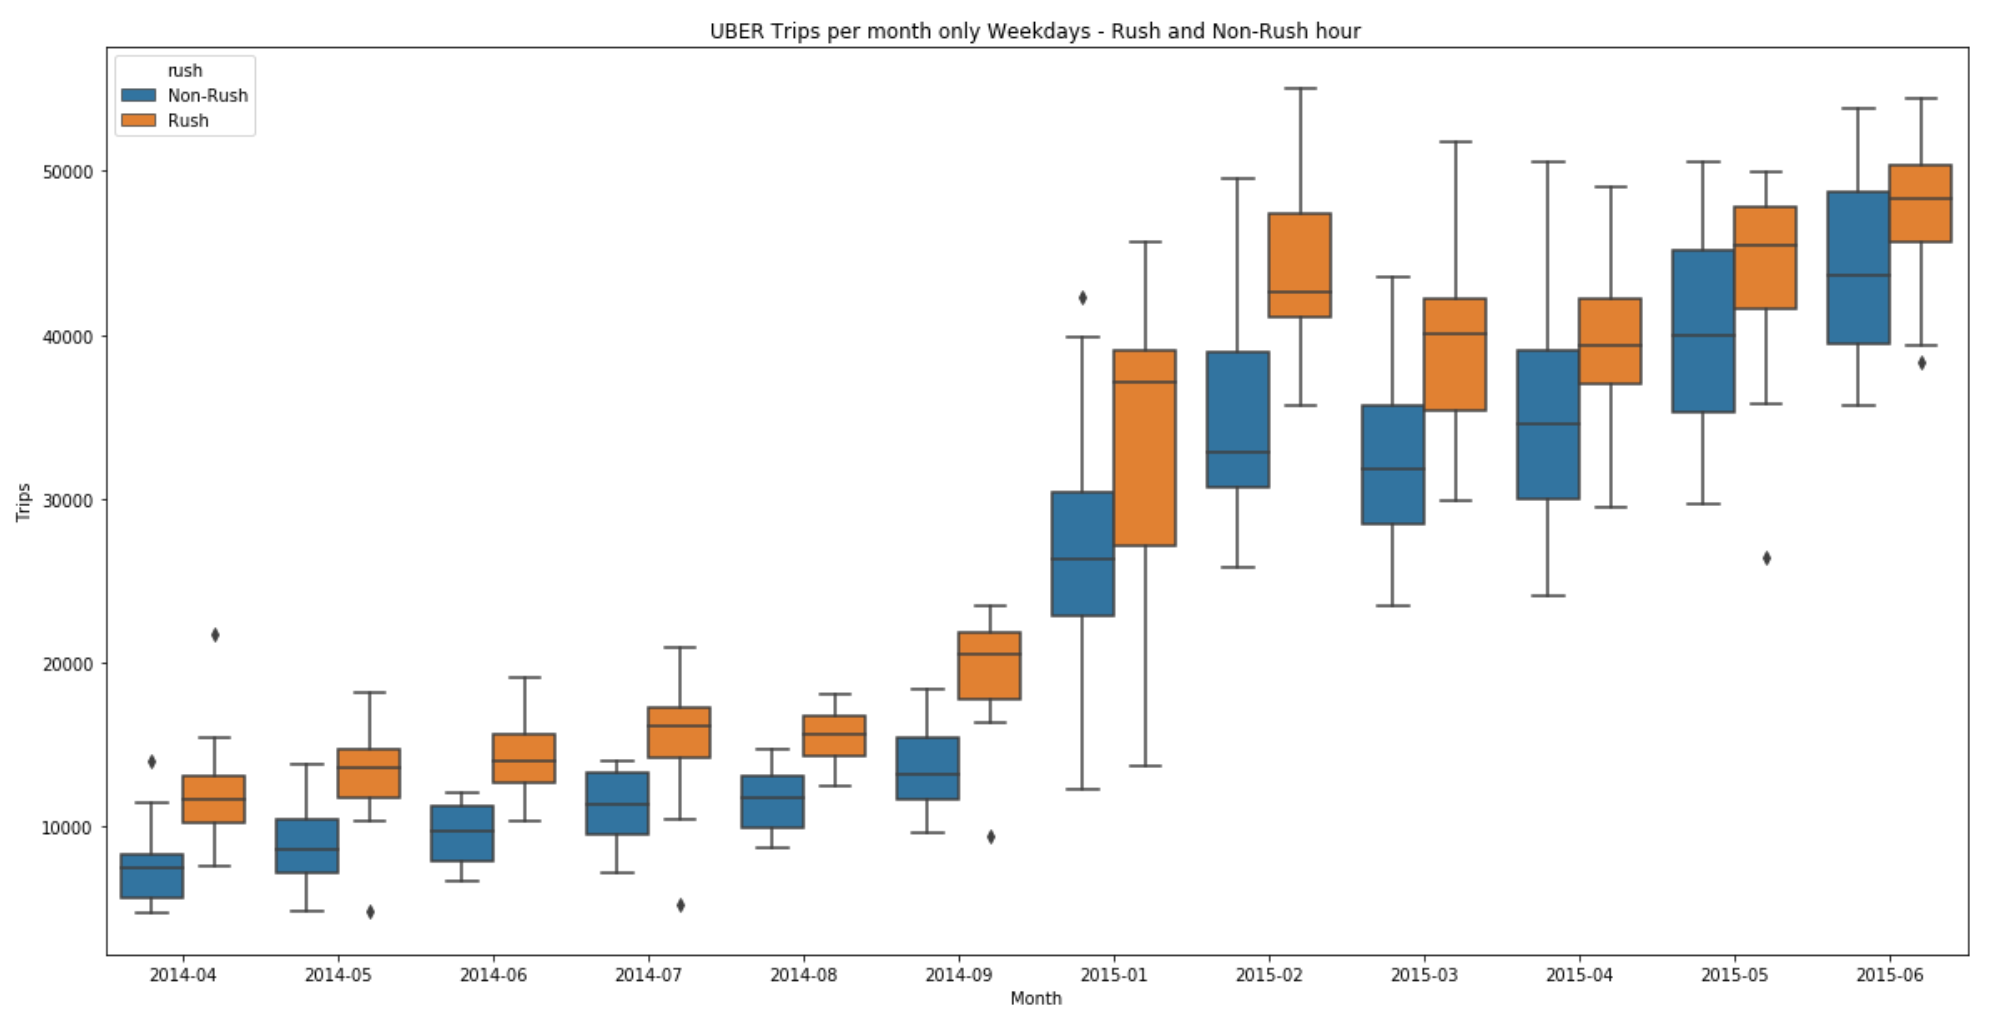
\includegraphics[height=2in, width=3.5in]{UBER_trips_only_weekdays_rush_and_non_rush.png}}%
\qquad
\subfigure[Yellow cab trips]{%
\label{fig:b}%
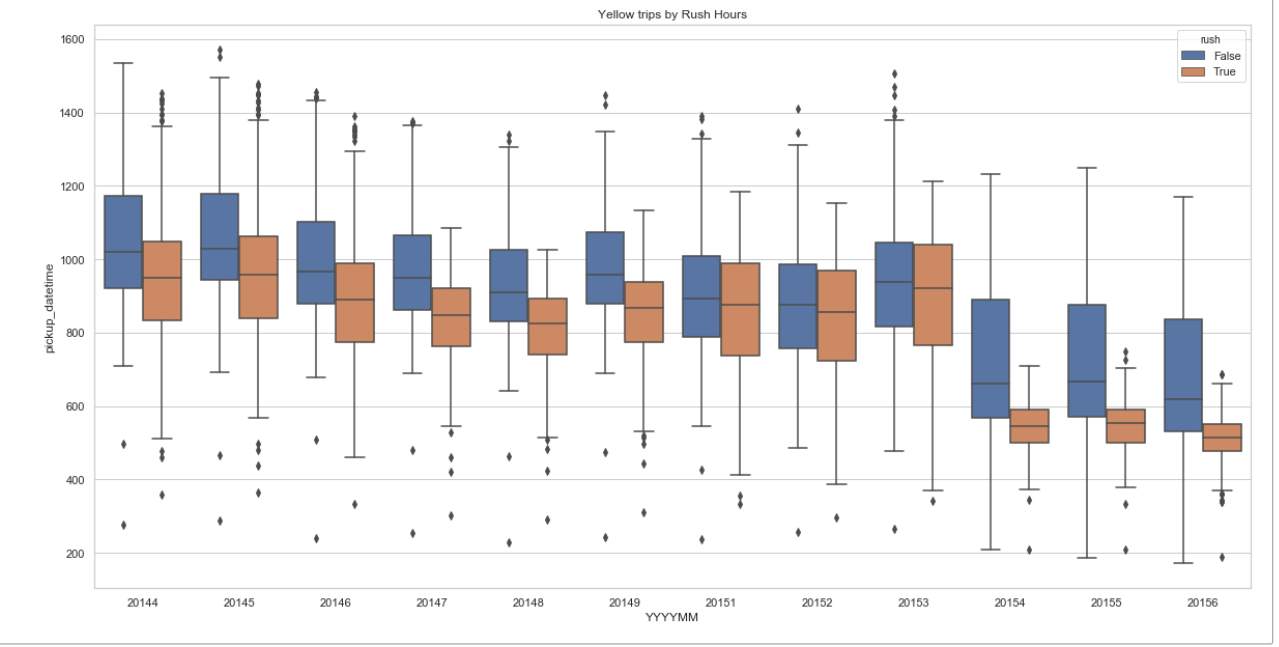
\includegraphics[height=2in, width=3.5in]{yellowTripsRushHours.png}}%
\qquad
\subfigure[Green cab trips]{%
\label{fig:c}%
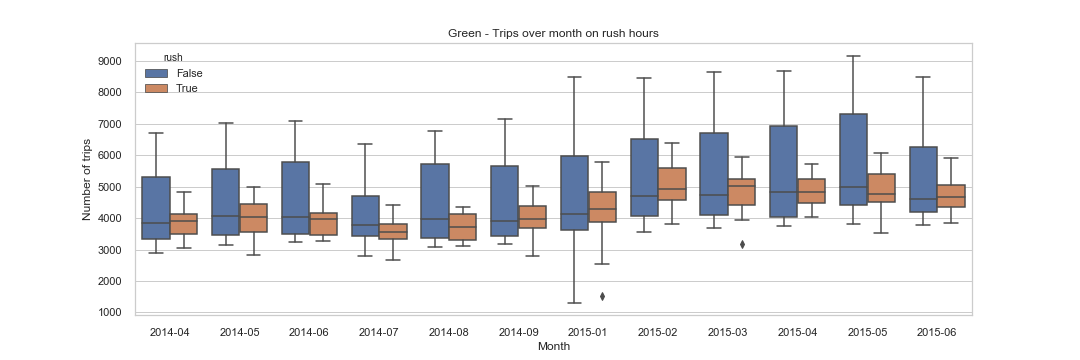
\includegraphics[height=2.4in, width=3.5in]{green_trips_month_rush.png}}%
\qquad
\subfigure[MTA trips]{%
\label{fig:d}%
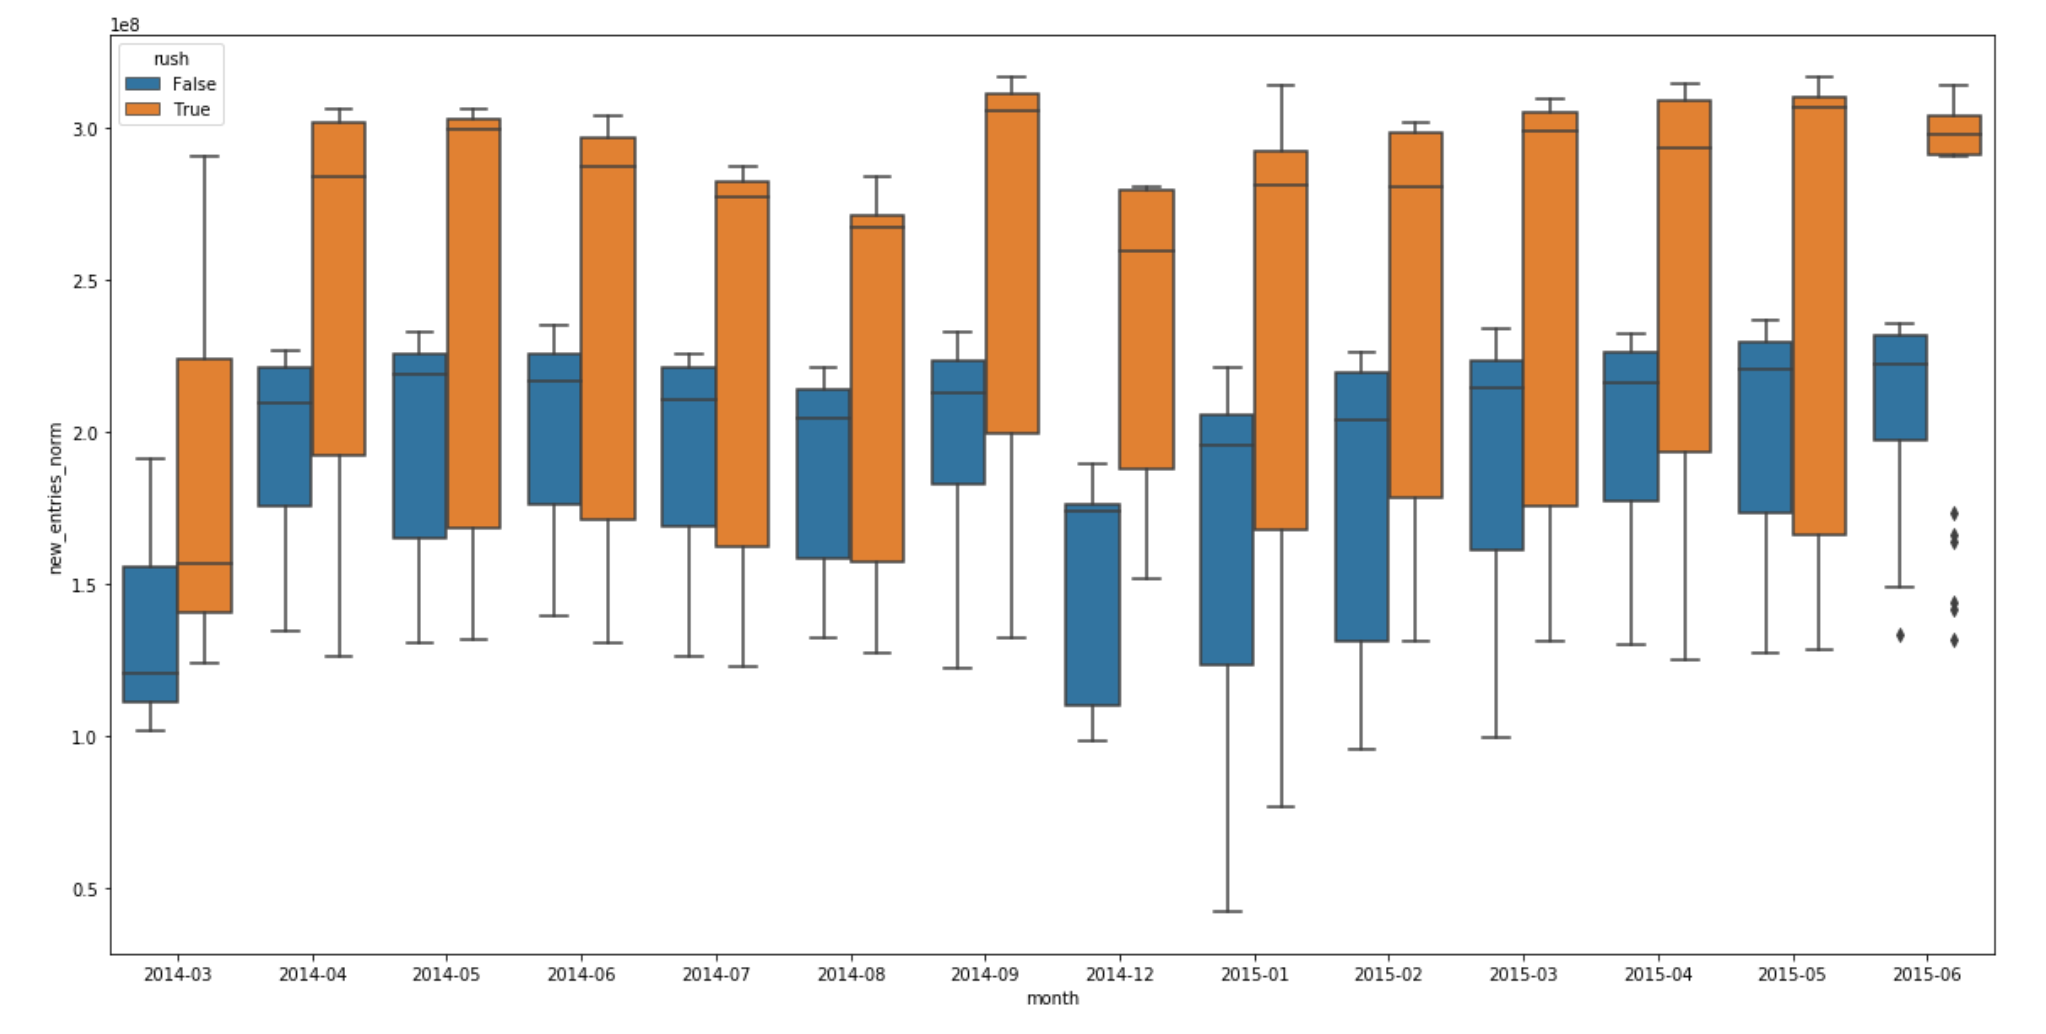
\includegraphics[height=2in, width=3.5in]{mta_new_entries_orange_rush_hour.png}}%
\caption{Has the increase of Uber trips affected the number of trips of Yellow cab, Green cab, and MTA trips? Orange boxes represent the number of trips in rush hours and blue ones correspond to non-rush hours. }
\label{fig:boxTrips}%
\end{figure}



Figure \ref{fig:boxDistances} compares the number of trips made by Uber with the monthly average travel distance covered by Yellow cabs. The aim of this comparison was to analyze if the increase of Uber trips affected the average travel distance of   plots, it is possible to see that from 2015, Uber is widely used for long distance trips, in contrast to Yellow cabs. On the other hand, the average travel distance of Yellow cabs experienced an increase in April 2015. 


%\begin{figure}%
%\centering
%\subfigure[Uber]{%
%\label{fig:first}%
%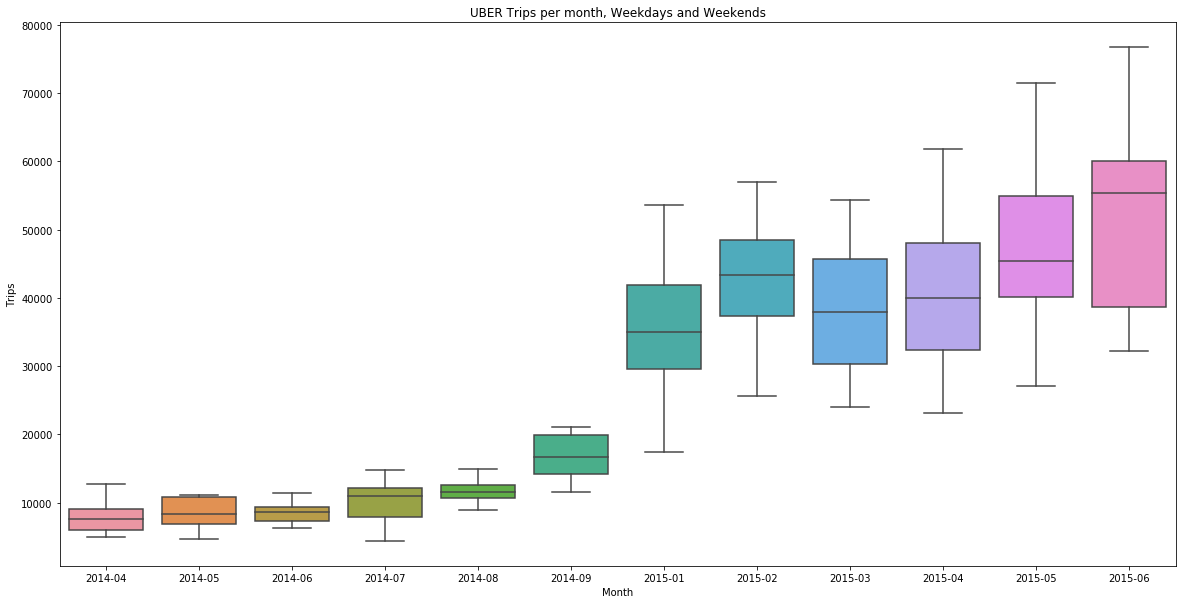
\includegraphics[height=2in, width=5in]{UBER_Trips_per_month_only_weekends.png}
%\qquad
%\subfigure[Yellow cabs]{%
%\label{fig:second}%
%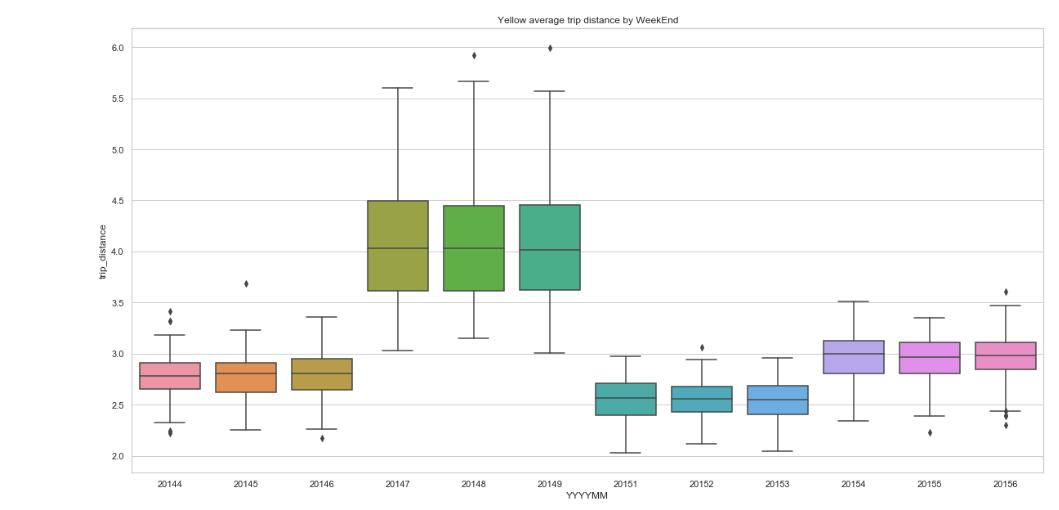
\includegraphics[height=2.2in, width=5.5in]{Yellow_Cabs_Average_trip_distance_Weekend_Only_by_Month_copy.png}}%
%\caption{Has the increase of Uber trips affected the average travel distance of Yellow cab trips? Comparison of the monthly number of trips performed by Uber and the monthly average travel distance covered by Yellow cabs. Yellow }
%\label{fig:boxDistances}%
%\end{figure}
%



\begin{figure}%
\centering
\subfigure[Uber trips.]{%
\label{fig:a}%
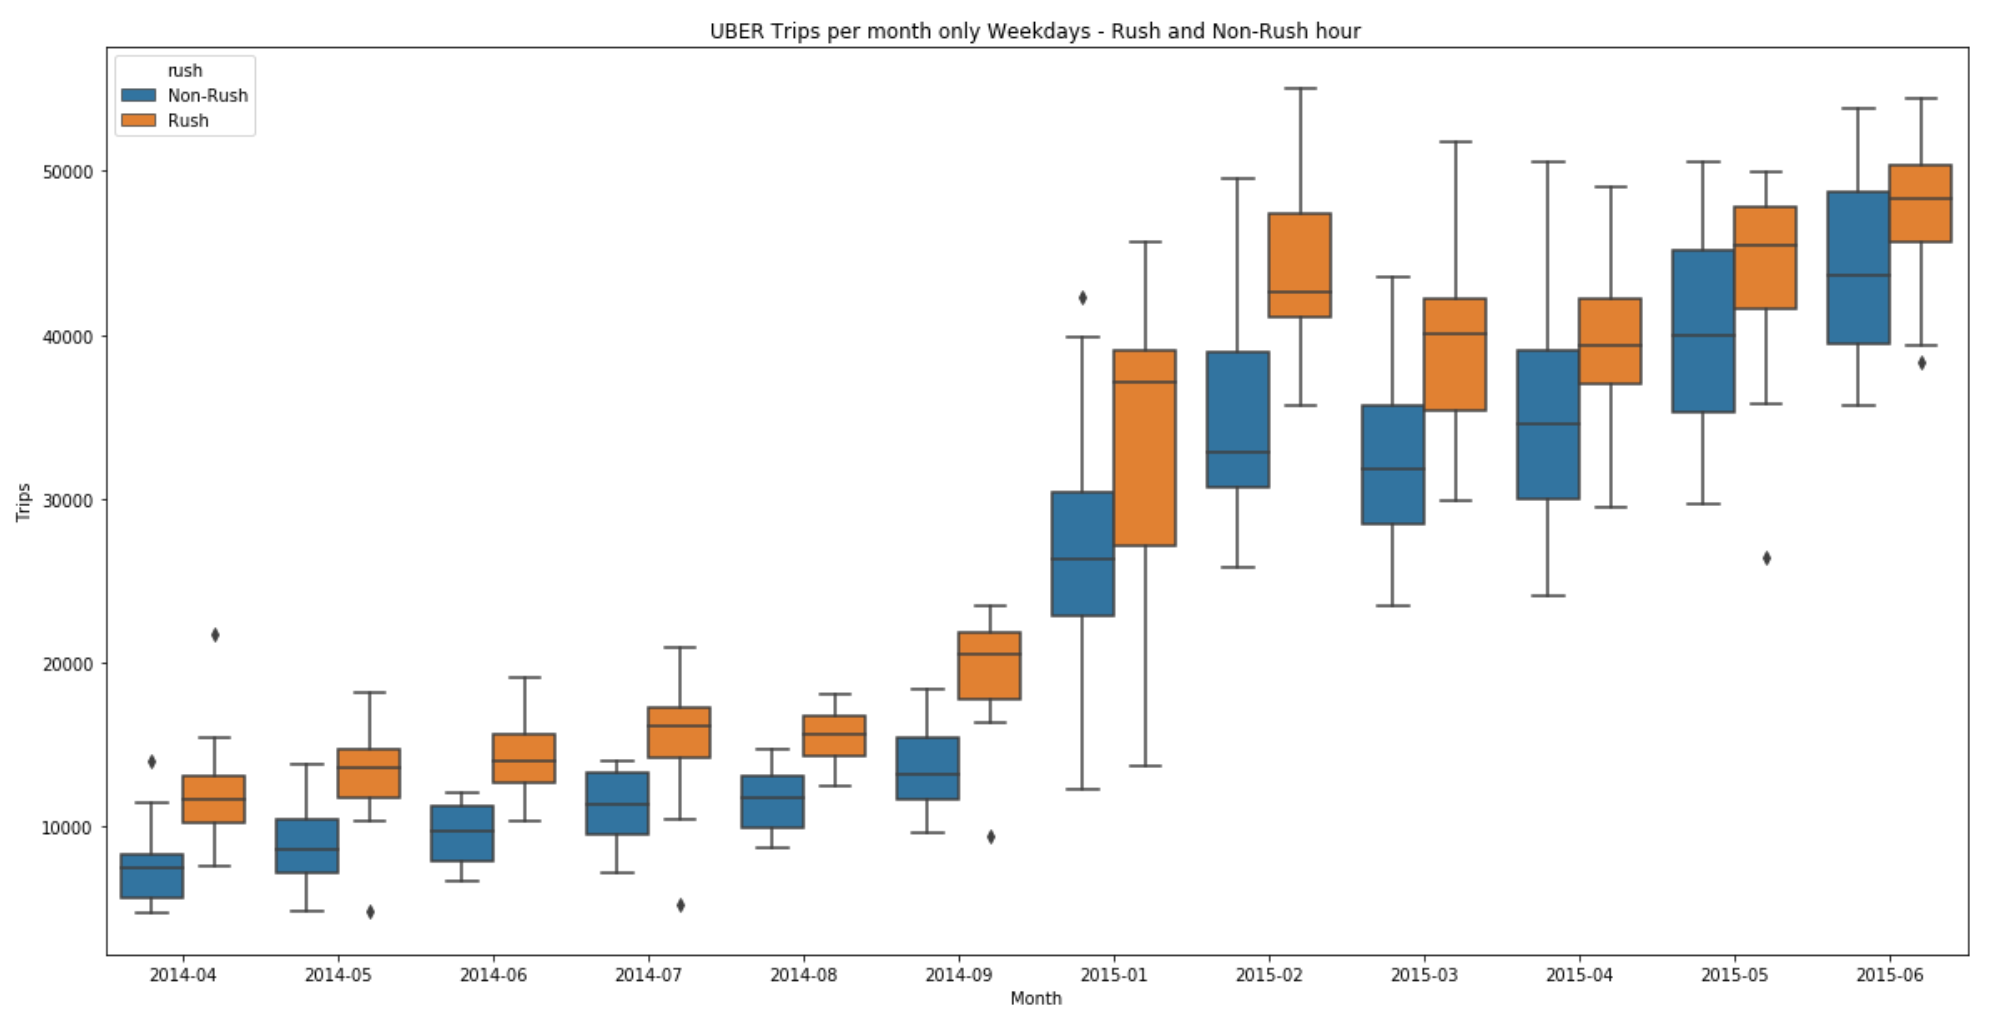
\includegraphics[height=2in, width=3.5in]{UBER_trips_only_weekdays_rush_and_non_rush.png}}%
\qquad
\subfigure[Yellow cab trips]{%
\label{fig:b}%
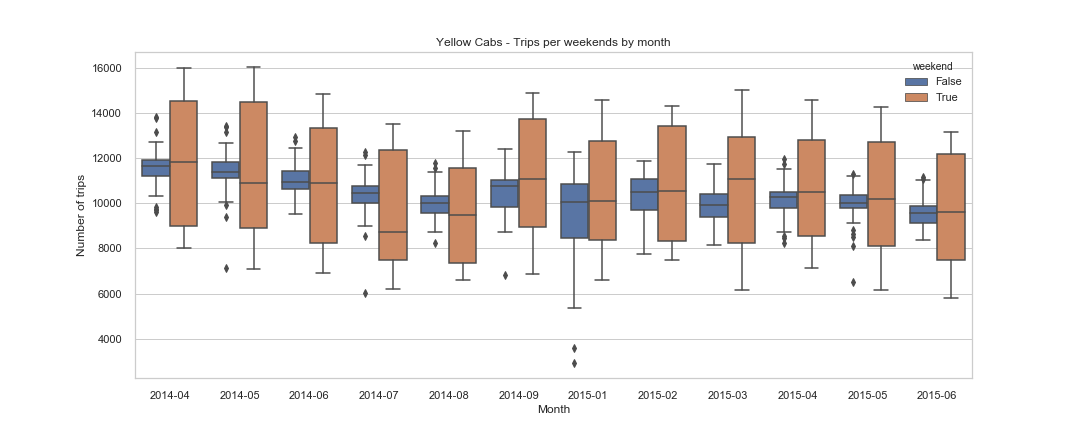
\includegraphics[height=2in, width=3.5in]{yellow_trips_month_weekend.png}}%
\qquad
\subfigure[Green cab trips]{%
\label{fig:c}%
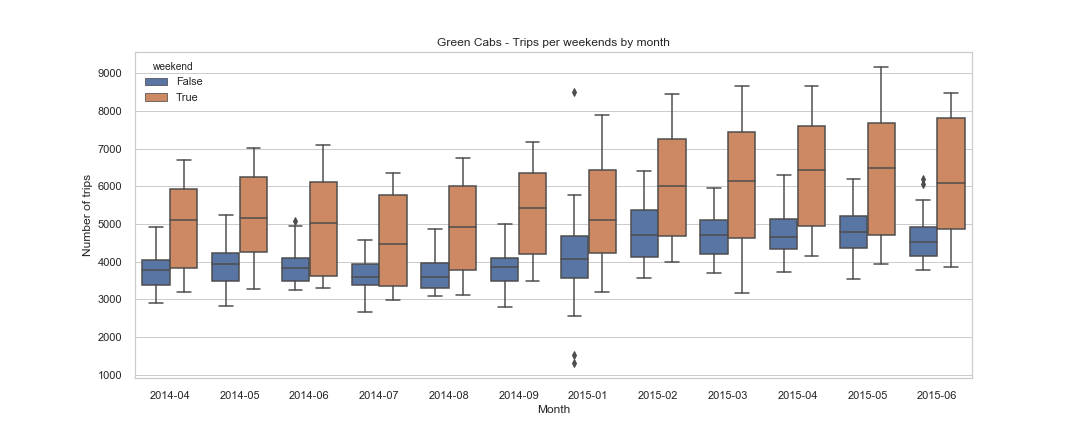
\includegraphics[height=2.4in, width=3.5in]{green_trips_month_weekend.png}}%
\qquad
\subfigure[MTA trips]{%
\label{fig:d}%
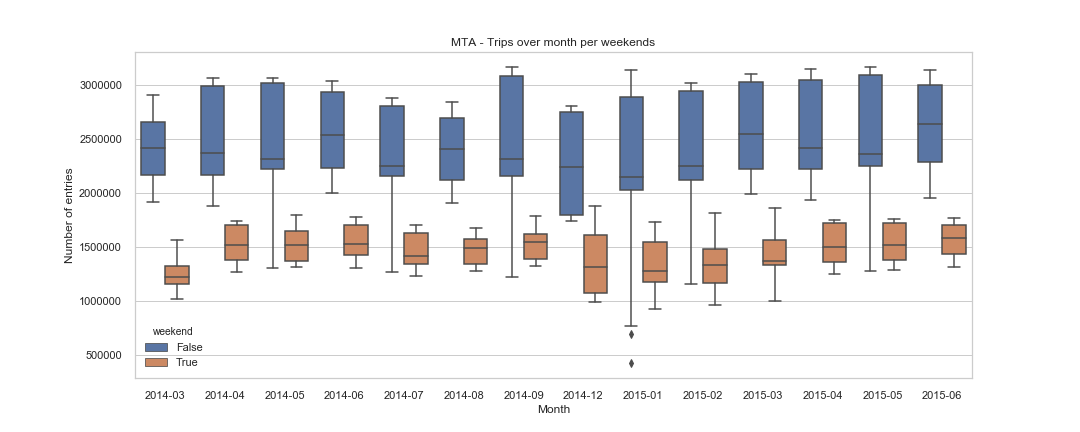
\includegraphics[height=2in, width=3.5in]{mta_entries_month_weekend.png}}%
\caption{trips weekend by month }
\label{fig:boxTrips}%
\end{figure}




\begin{figure}%
\centering
\subfigure[Uber trips.]{%
\label{fig:a}%
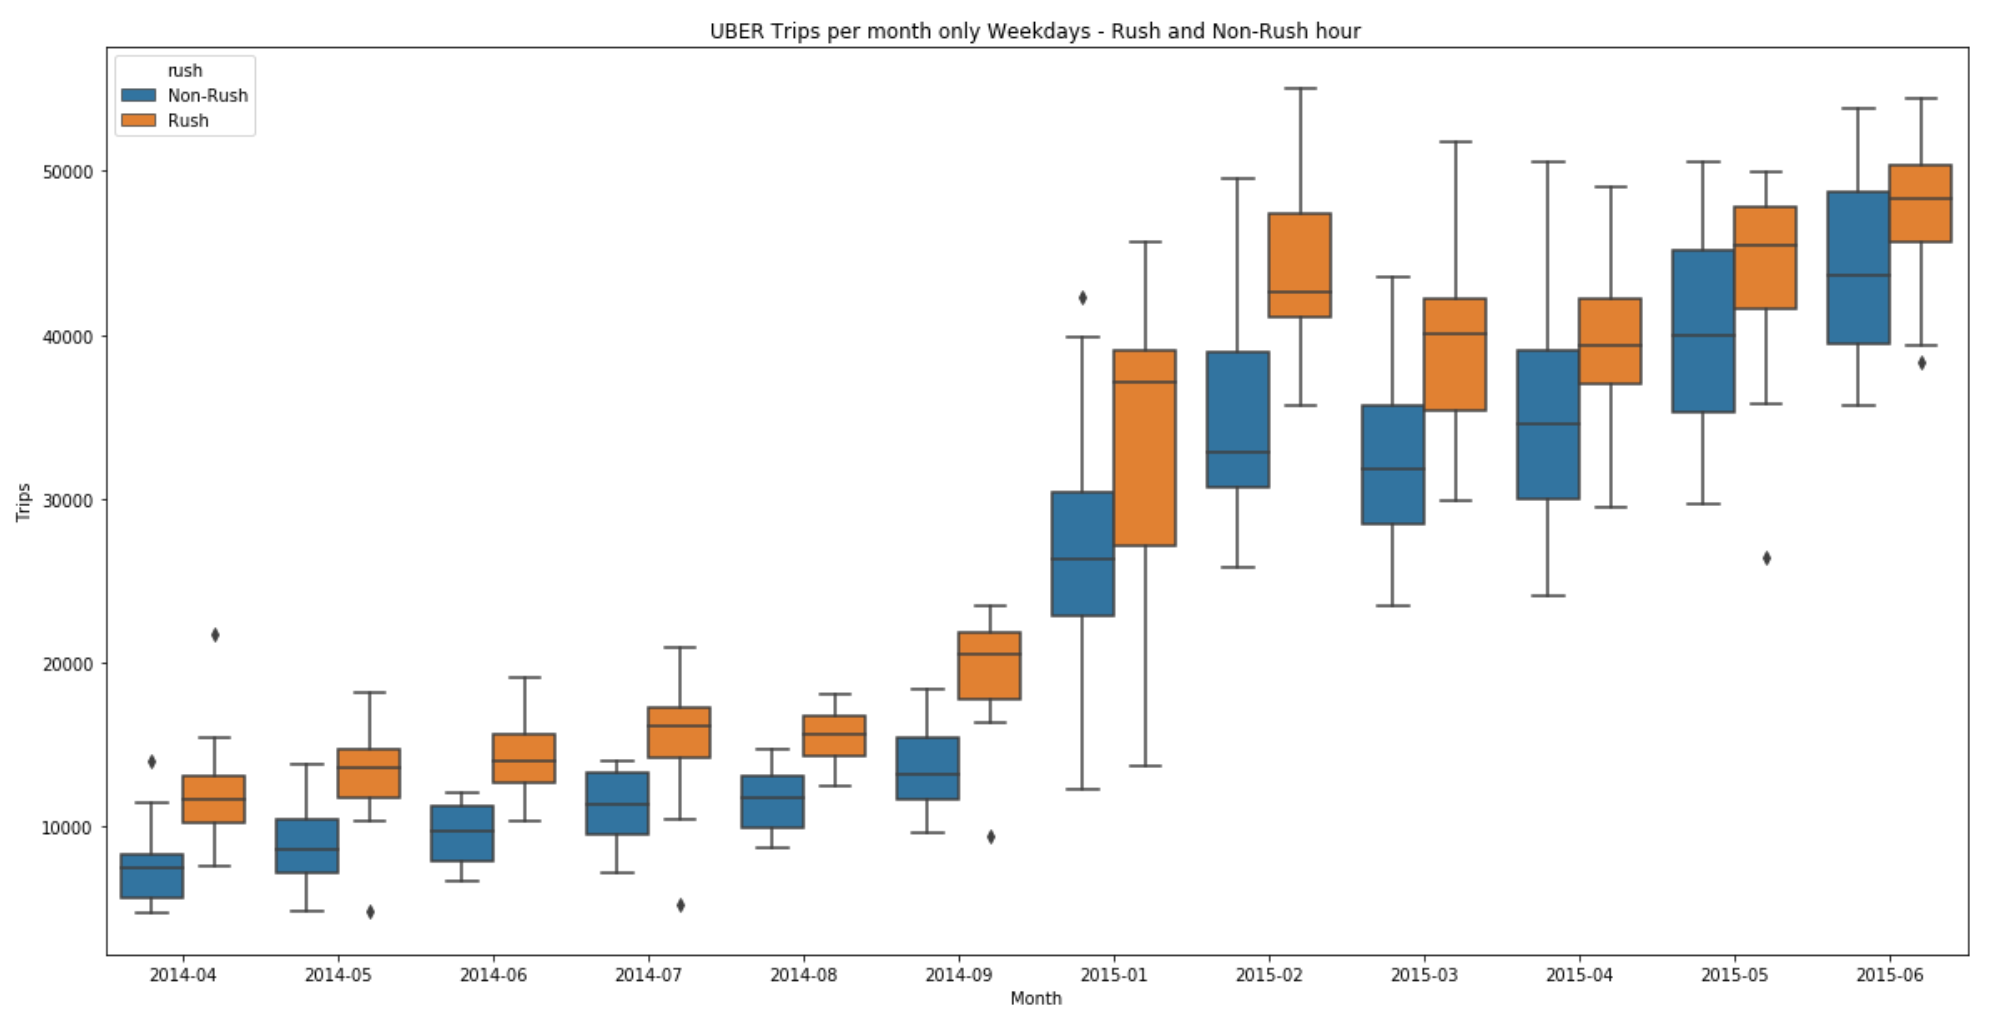
\includegraphics[height=2in, width=3.5in]{UBER_trips_only_weekdays_rush_and_non_rush.png}}%
\qquad
\subfigure[Yellow cab trips]{%
\label{fig:b}%
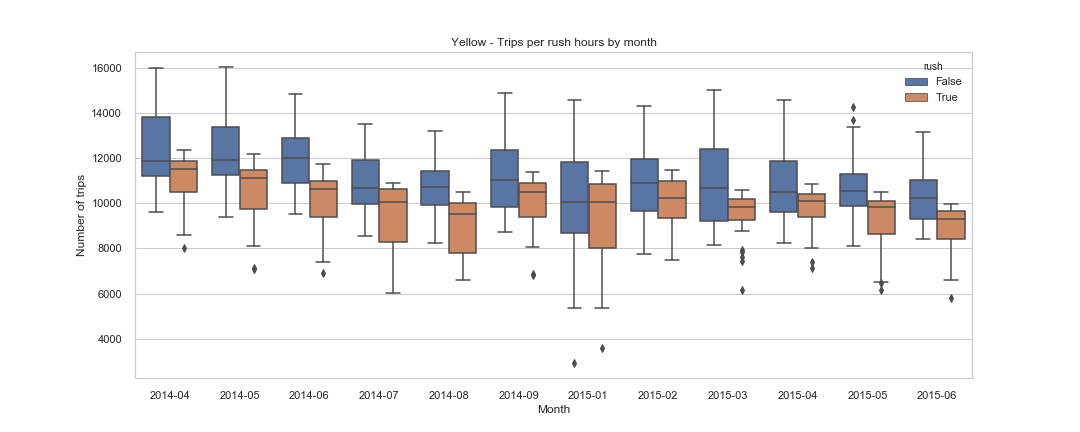
\includegraphics[height=2in, width=3.5in]{yellow_trips_month_rush.png}}%
\qquad
\subfigure[Green cab trips]{%
\label{fig:c}%
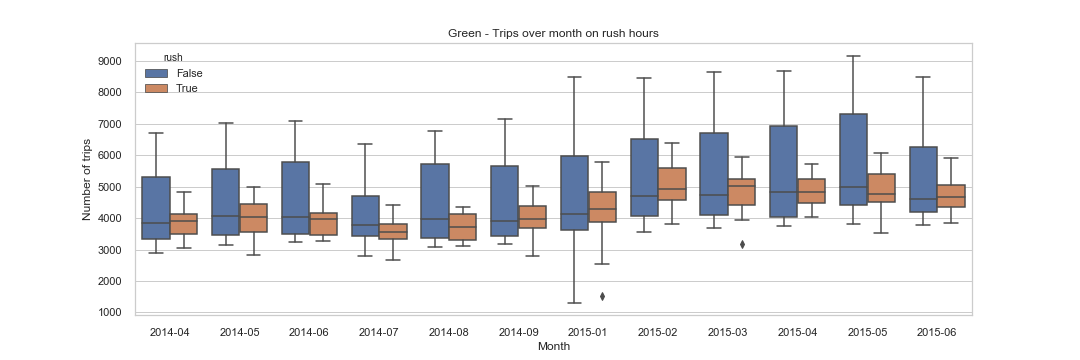
\includegraphics[height=2.4in, width=3.5in]{green_trips_month_rush.png}}%
\qquad
\subfigure[MTA trips]{%
\label{fig:d}%
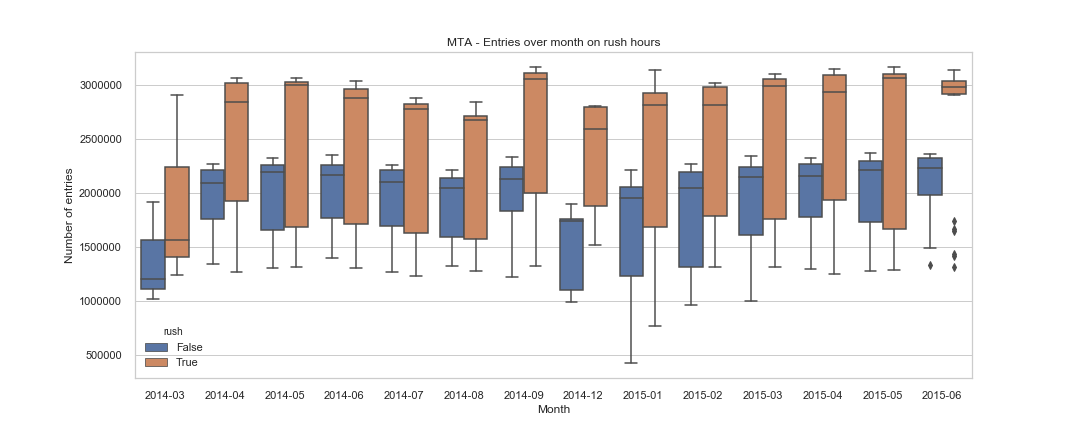
\includegraphics[height=2in, width=3.5in]{mta_entries_month_rush.png}}%
\caption{trips month rush hours }
\label{fig:boxTrips}%
\end{figure}




\begin{figure}%
\centering
\subfigure[Uber trips.]{%
\label{fig:a}%
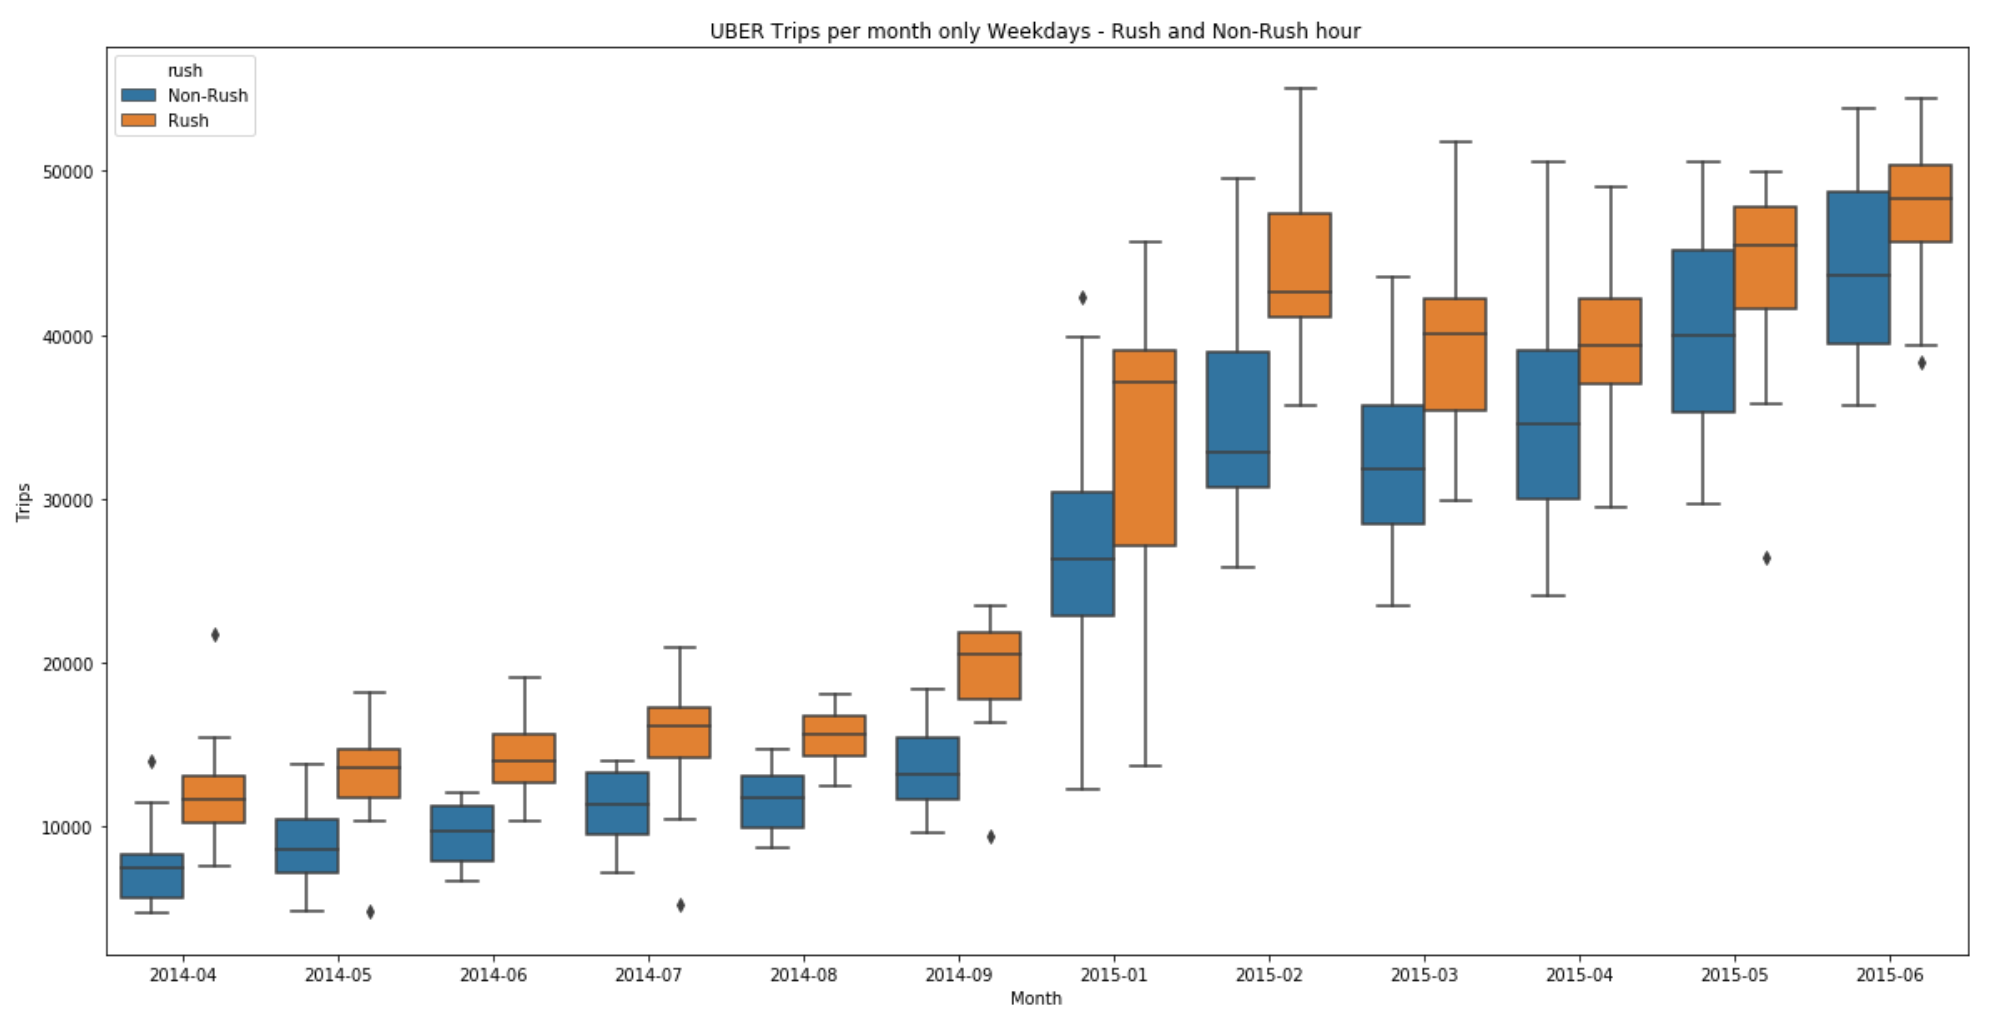
\includegraphics[height=2in, width=3.5in]{UBER_trips_only_weekdays_rush_and_non_rush.png}}%
\qquad
\subfigure[Yellow cab trips]{%
\label{fig:b}%
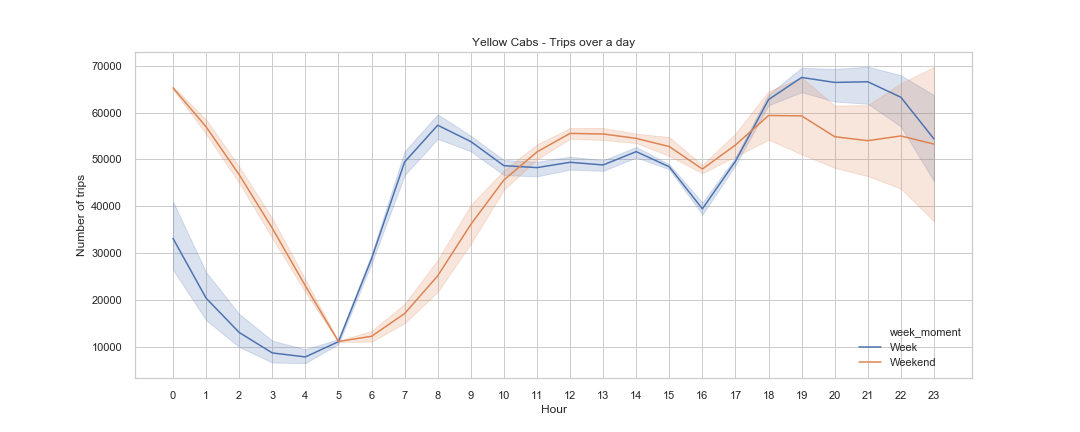
\includegraphics[height=2in, width=3.5in]{yellow_trips_hour_week.png}}%
\qquad
\subfigure[Green cab trips]{%
\label{fig:c}%
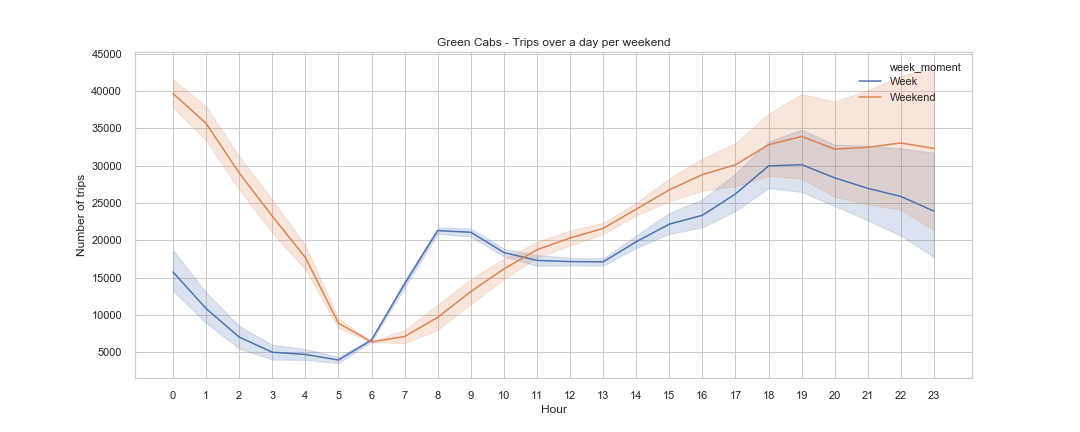
\includegraphics[height=2.4in, width=3.5in]{green_trips_hour_week.png}}%
\qquad
\subfigure[MTA trips]{%
\label{fig:d}%
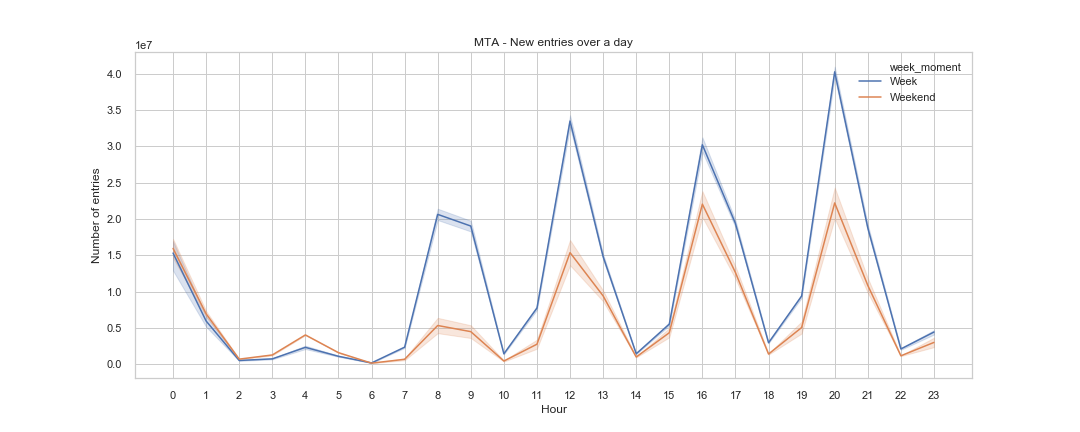
\includegraphics[height=2in, width=3.5in]{mta_entries_hour_week.png}}%
\caption{Hour week }
\label{fig:boxTrips}%
\end{figure}


%
%
%\begin{figure}%
%\centering
%\subfigure[Uber trips.]{%
%\label{fig:a}%
%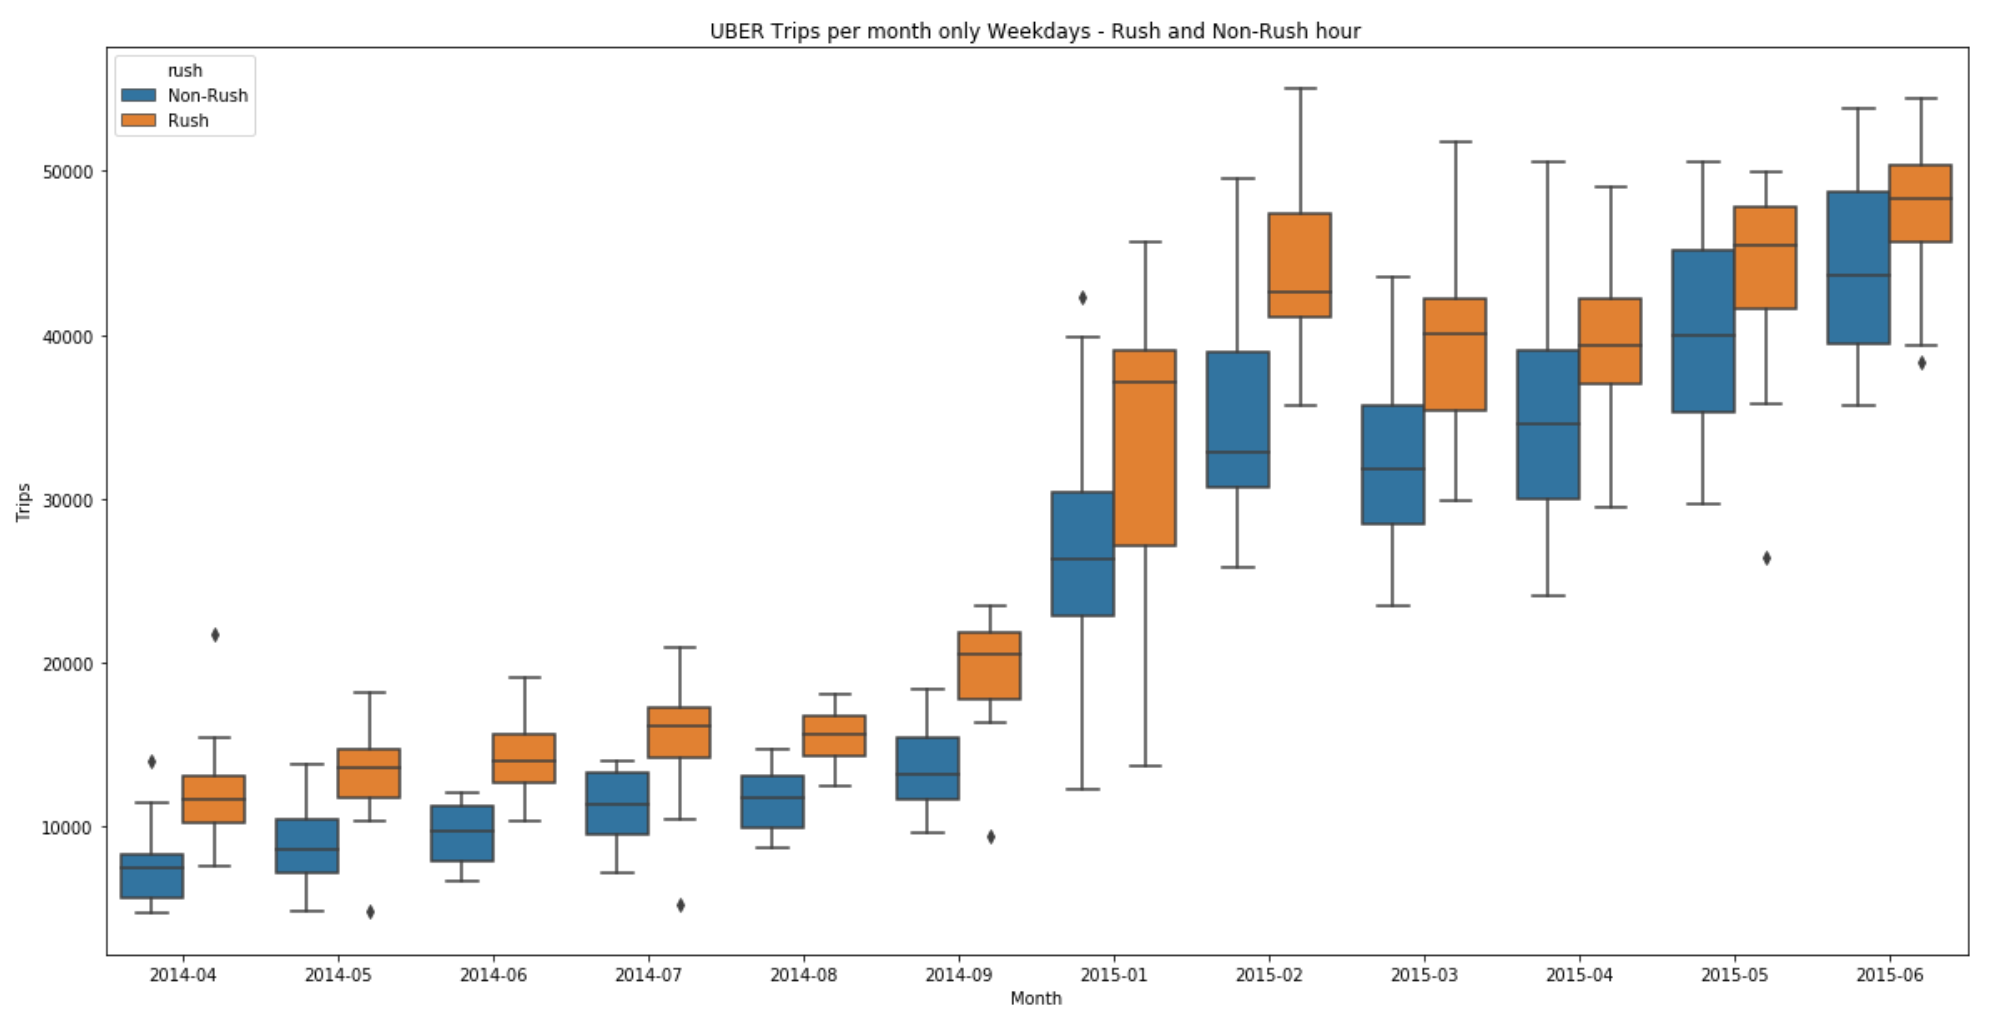
\includegraphics[height=2in, width=3.5in]{UBER_trips_only_weekdays_rush_and_non_rush.png}}%
%\qquad
%\subfigure[Yellow cab trips]{%
%\label{fig:b}%
%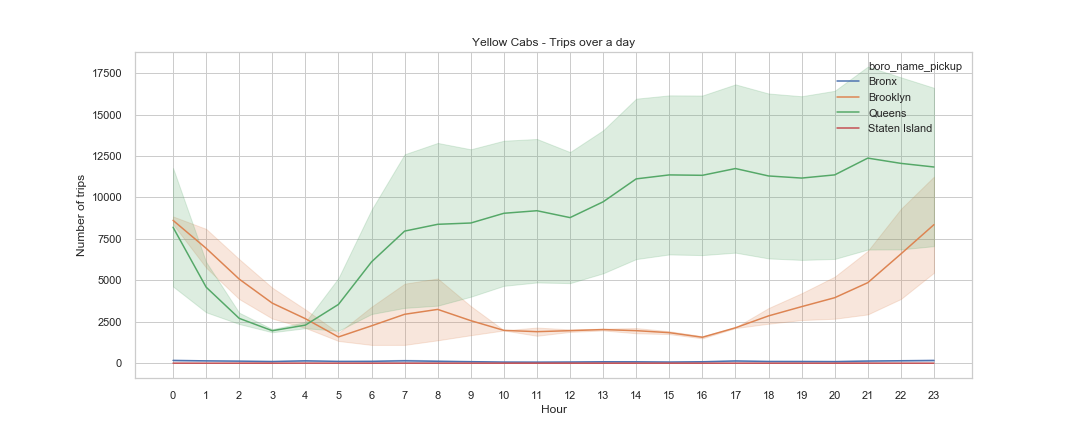
\includegraphics[height=2in, width=3.5in]{yellow_trips_hour_borough.png}}%
%\qquad
%\subfigure[Green cab trips]{%
%\label{fig:c}%
%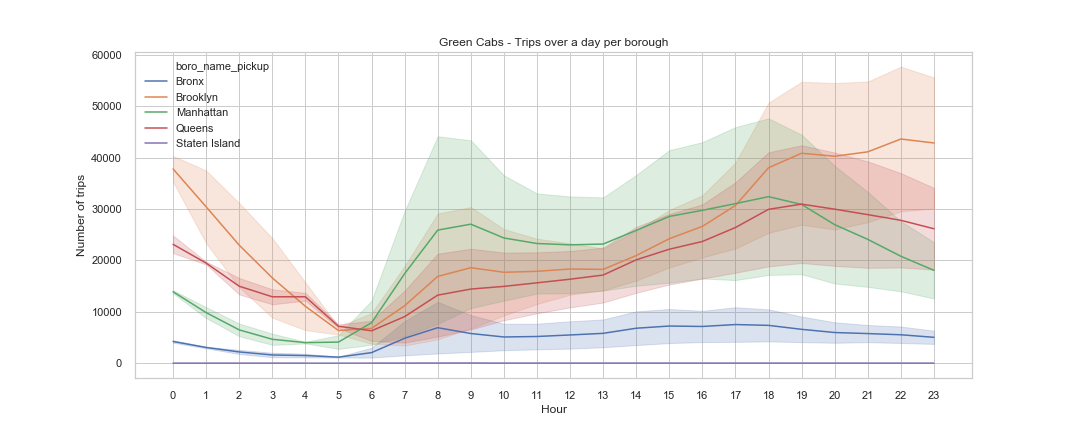
\includegraphics[height=2.4in, width=3.5in]{green_trips_hour_borough.png}}%
%\qquad
%\subfigure[MTA trips]{%
%\label{fig:d}%
%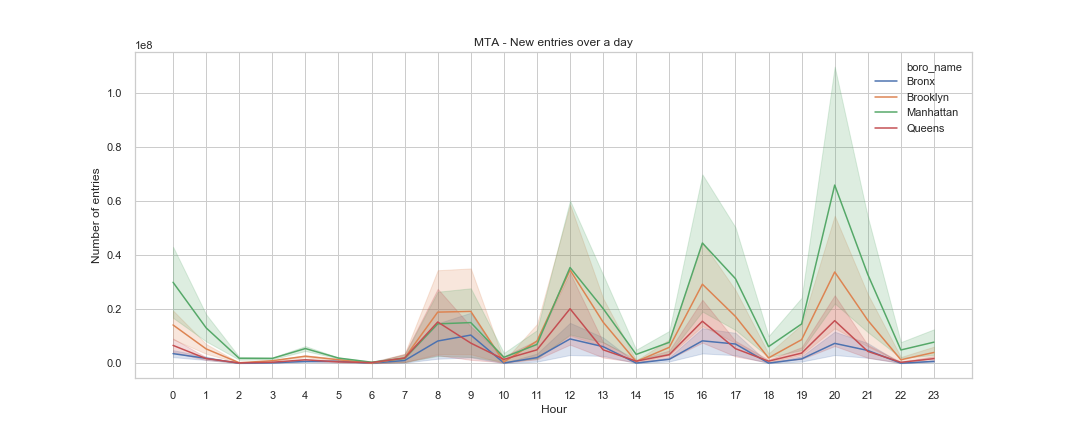
\includegraphics[height=2in, width=3.5in]{mta_entries_hour_borough.png}}%
%\caption{Hour borough }
%\label{fig:boxTrips}%
%\end{figure}




\begin{figure}%
\centering
\subfigure[Uber trips.]{%
\label{fig:a}%
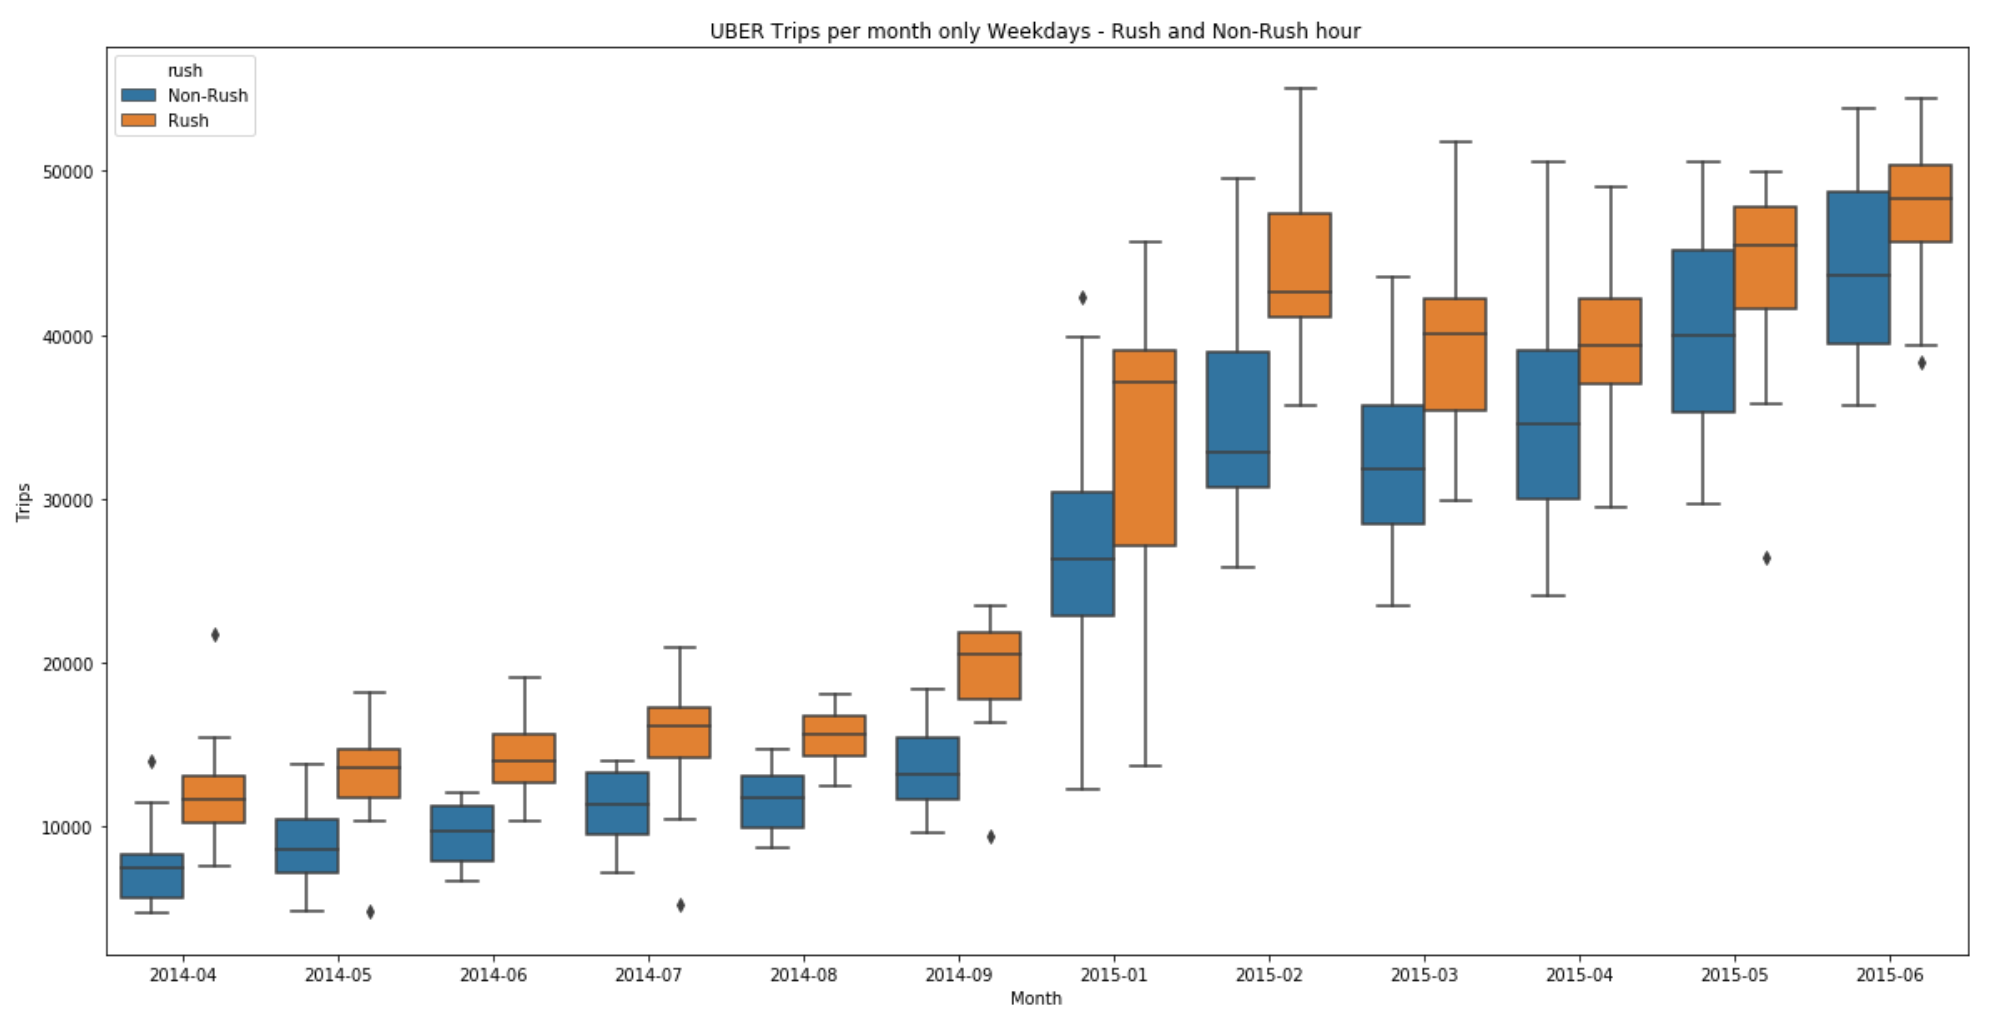
\includegraphics[height=2in, width=4in]{UBER_trips_only_weekdays_rush_and_non_rush.png}}%
\qquad
\subfigure[Yellow cab trips]{%
\label{fig:b}%
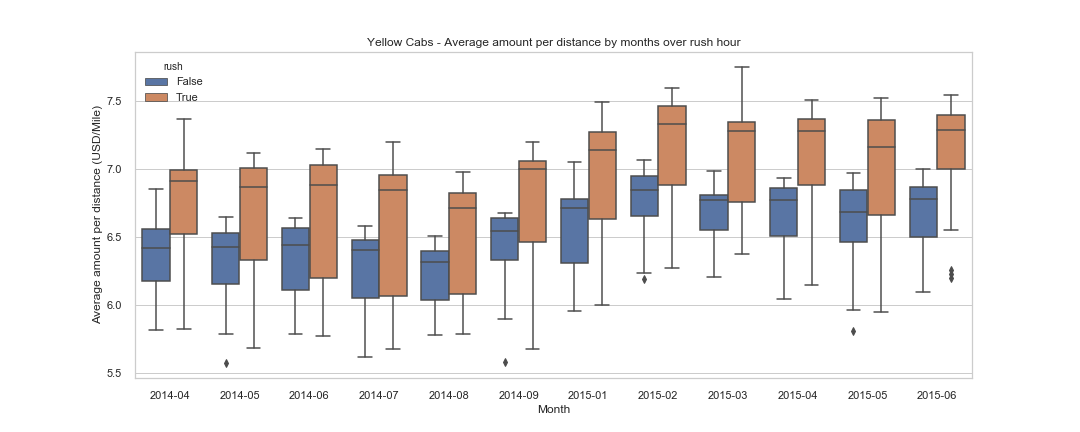
\includegraphics[height=2in, width=4in]{yellow_avgamountperdistance_rush_month_boxplot.png}}
\qquad
\subfigure[Green cab trips]{%
\label{fig:c}%
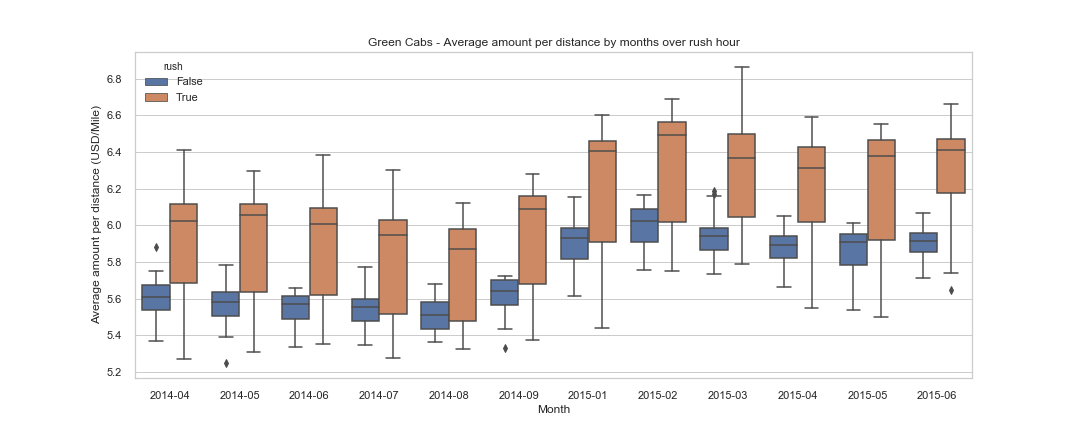
\includegraphics[height=2.4in, width=4in] {green_avgamountperdistance_rush_month_boxplot.png}}%
\caption{price per distance }
\label{fig:boxTrips}%
\end{figure}


\begin{figure}%
\centering
\subfigure[Uber trips.]{%
\label{fig:a}%
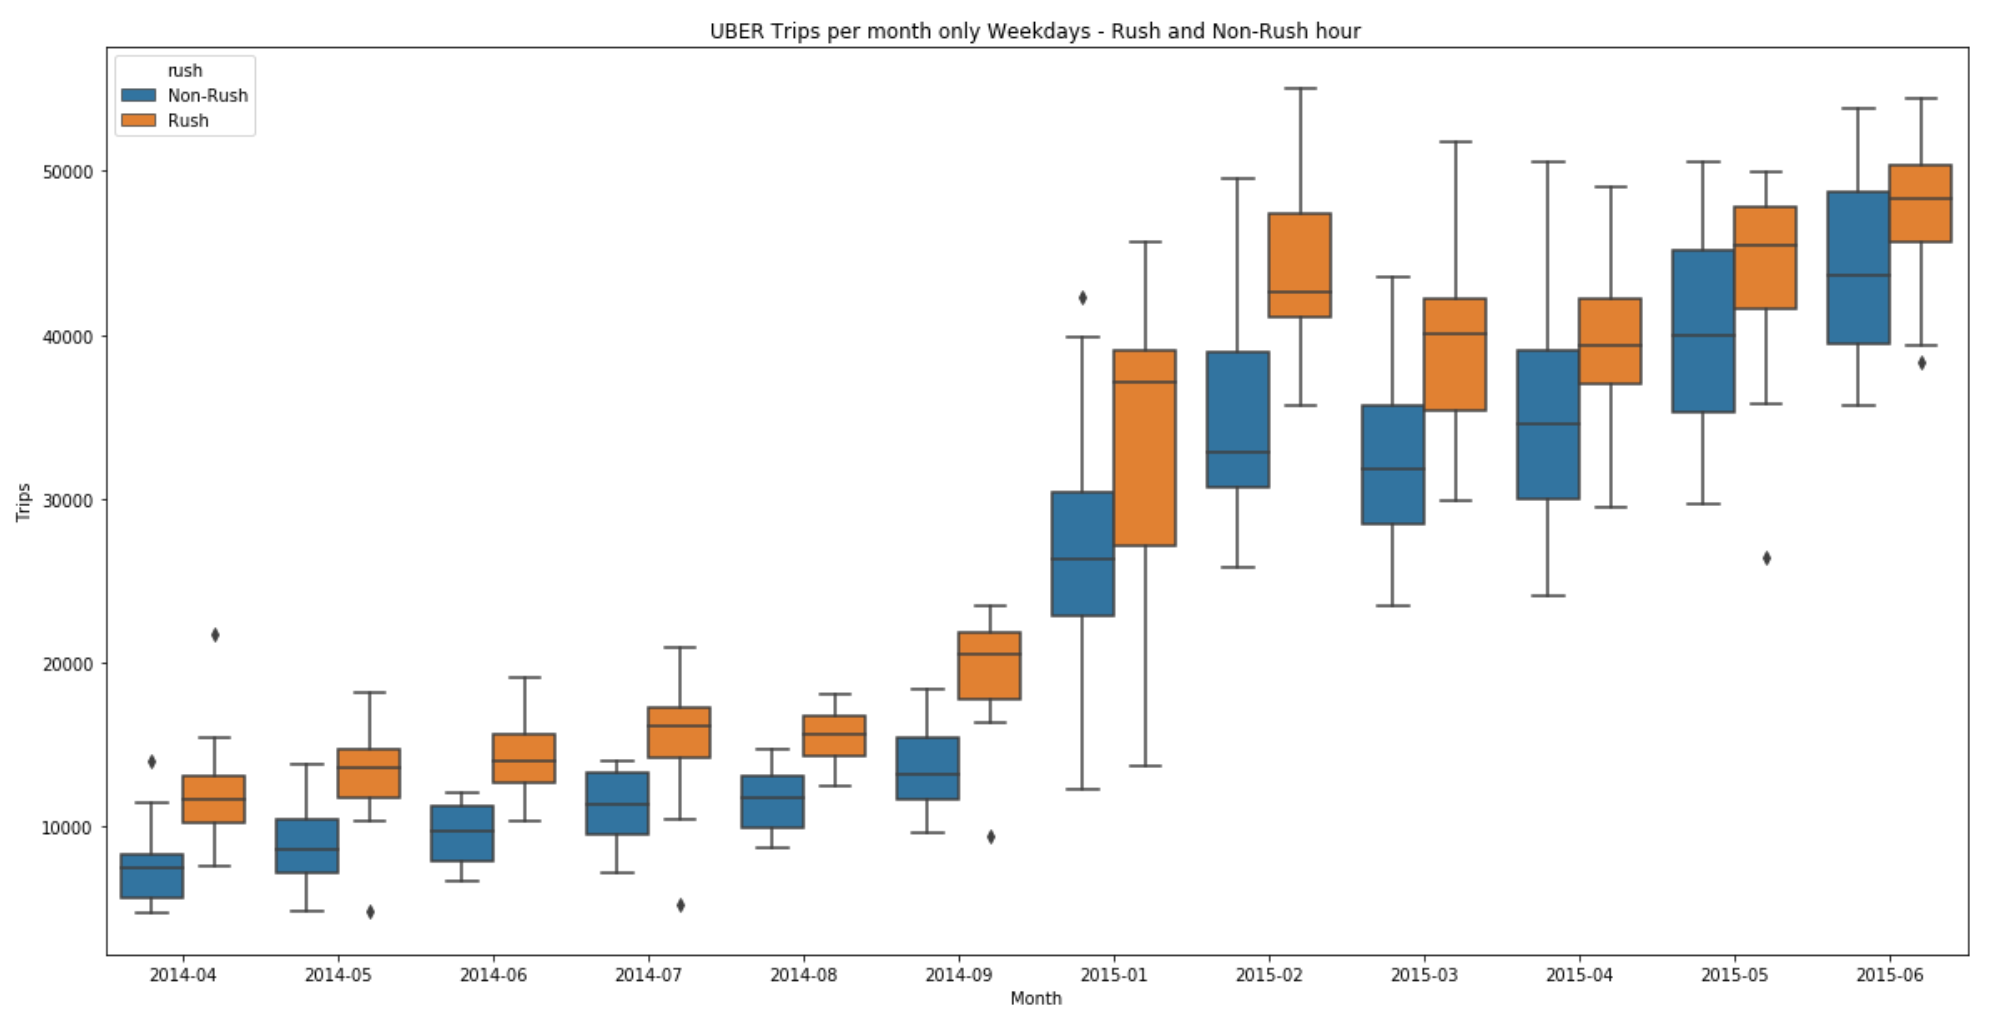
\includegraphics[height=2in, width=4in]{UBER_trips_only_weekdays_rush_and_non_rush.png}}%
\qquad
\subfigure[Yellow cab trips]{%
\label{fig:b}%
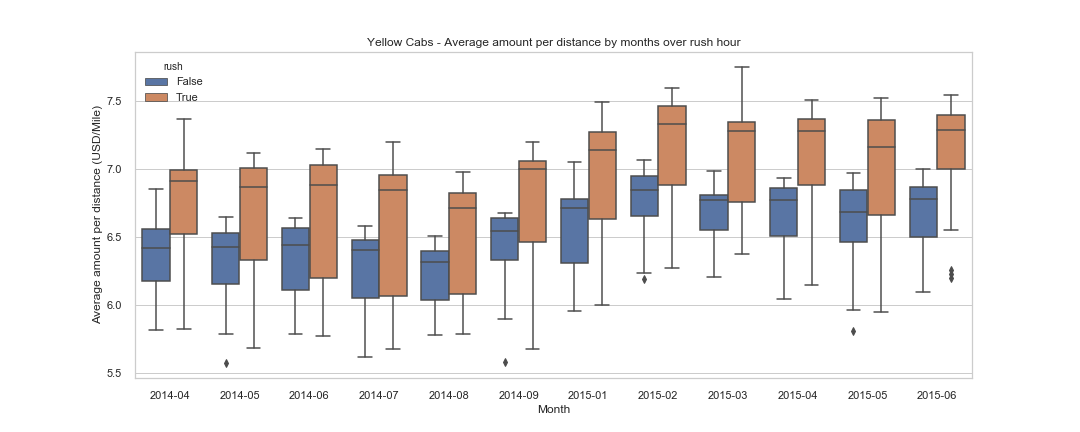
\includegraphics[height=2in, width=4in]{yellow_avgamountperdistance_rush_month_boxplot.png}}
\qquad
\subfigure[Green cab trips]{%
\label{fig:c}%
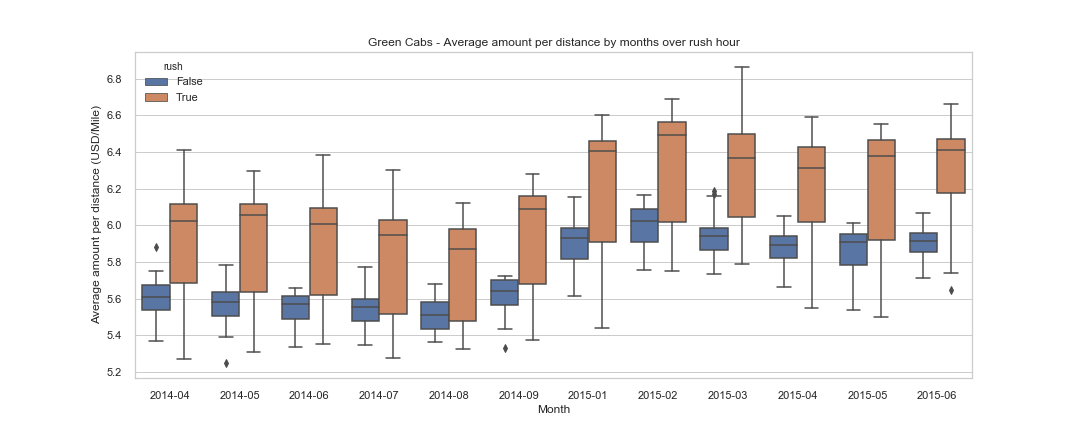
\includegraphics[height=2.4in, width=4in] {green_avgamountperdistance_rush_month_boxplot.png}}%
\caption{avrg distance }
\label{fig:boxTrips}%
\end{figure}




%\section{Statistical Analysis and Modeling}
\label{sec:datAnalisys}
What assumptions and choices did your team make, and
what was your justification for them? How did you perform feature selection? If you built
models, how did you analyze their performance, and what shortcomings do they exhibit?
If you constructed visualizations and/or conducted statistical tests, what was the
motivation behind the particular ones you built?
%\section{Results Interpretation and Conclusions}
\label{sec:results}
What were your team?s key findings, and what is
their significance? Are your conclusions precise and nuanced, as opposed to blanket
(over)generalizations? You should use summary statistics and visualizations to help
explain your thoughts.



%\begin{table}[h]
%\begin{center}
%\label{tabDataset}
%\begin{tabular}{|c|c|c|c|c|}
%\hline
%\textbf{Data Name} & \textbf{Description} & \textbf{Type} & \textbf{Number} & \textbf{Database}   \\
%\hline
% Event name: & type of disaster (flooding,XX)& categorical &S &  UNGRD\\
% Date: & incident date & numerical &XXX &  UNGRD/DANE  \\
% Code: &disaster ID & numerical &XXX &  UNGRD/DANE  \\
% Municipality Code: & Divipol code & numerical &XXX &  UNGRD/DANE  \\
% Dead: & Deads per incident & numerical &XXX &  UNGRD  \\
% Wounded: & Wound per incident & numerical &XXX &  UNGRD  \\
% Disappeared: & Disappeared per incident & numerical &XXX &  UNGRD  \\
%  Affected: & Affected people & numerical &XXX &  UNGRD  \\
%   Affected families: & Affected people & numerical &XXX &  UNGRD  \\
%\hline
%\end{tabular}
% \caption{Summary of the main information available to develop the project.}
%\end{center}
%\end{table}


\bibliographystyle{abbrv}
\bibliography{simple}

\end{document}
This is never printed
